%% -*- ispell-local-dictionary: "italiano" -*-
%% Local Variables:
%% ispell-local-dictionary: "italiano"
%% eval: (flyspell-mode 1)
%% End:


\documentclass[a4paper, 12pt]{article}

\usepackage[utf8]{inputenc}
\usepackage[T1]{fontenc}
\usepackage{lipsum}
\usepackage{parskip}
\usepackage[a4paper,width=150mm,top=25mm,bottom=25mm]{geometry}

\usepackage{amsmath}
\usepackage{graphicx}
\usepackage{float}
\usepackage{subcaption}
\captionsetup{width=0.8\textwidth}

\usepackage{listings}
\usepackage{xcolor}
\lstset{
  basicstyle=\ttfamily,
  columns=fullflexible,
  breaklines=true,
  postbreak=\raisebox{0ex}[0ex][0ex]{\color{red}$\hookrightarrow$\space},
  keepspaces,
  language=Bash,
  showtabs=true,
}

\usepackage[noframe]{showframe}
\usepackage{framed}
\renewenvironment{shaded}{%
  \def\FrameCommand{\fboxsep=\FrameSep \colorbox{shadecolor}}%
  \MakeFramed{\advance\hsize-\width \FrameRestore\FrameRestore}}%
 {\endMakeFramed}
 \definecolor{shadecolor}{gray}{0.90}

\usepackage{hyperref}
\hypersetup{
  colorlinks=false,
  hidelinks=true,
  pdftitle={Compressione di immagini tramite la DCT}
}

\usepackage[T1]{fontenc}
\usepackage{titlesec,  color}
\usepackage{fix-cm}
\makeatletter
\newcommand\HUGE{\@setfontsize\Huge{50}{60}}
\makeatother
\titleformat{\chapter}
	{\scshape\LARGE\bfseries\HUGE}
	{\makebox[6pc][l]{\HUGE\thechapter\hfil\rule[-4pt]{0.5pt}{2pc}}}
	{0pt}
	{\LARGE}
	\titlespacing*{\chapter}{0pt}{0pt}{24pt}


\title{\textsc{\textbf{Compressione di immagini tramite la DCT}}}

\author{
		\begin{tabular}{cc}
				Lorenzo Olearo & Alessandro Riva \\
				\href{mailto:l.olearo@campus.unimib.it}{\texttt{\small{l.olearo@campus.unimib.it}}} &
				\href{mailto:a.riva86@campus.unimib.it}{\texttt{\small{\quad a.riva86@campus.unimib.it}}}
		\end{tabular}
}



\date{A.A. 2022-2023}


\begin{document}
\maketitle


\textit{Lo scopo di questo progetto è di utilizzare l'implementazione della trasformata
	DCT2 in un ambiente open source e di studiare gli effetti di un algoritmo di
	compressione di tipo JPEG (senza utilizzare una matrice di quantizzazione) sulle
	immagini in toni di grigio. Comprende l'implementazione di un codice e la
	scrittura di una relazione da consegnare al docente.}

\vspace{12pt}

\begin{shaded}
Tutto il codice sorgente per il la realizzazione del progetto comprendente
consegne, test, esperimenti, grafici e relazione è stato pubblicato al seguente
repository GitHub: \url{https://github.com/LorenzoOlearo/cosine-image-compression}.
Il repository rimarrà privato fino alla data dell'esame, per avere l'accesso,
le chiediamo per ragioni tecniche di comunicarcelo via mail.
\end{shaded}

% \renewcommand{\contentsname}{Indice dei contenuti}
% \tableofcontents


\section{Confronto tra DCT diretta e veloce}
Nella prima parte del progetto si richiede di confrontare le prestazioni della
DCT2 come spiegata a lezione nella sua forma diretta, con quella di una libreria
open source a scelta che si presuppone essere nella sua versione \textit{fast}.

La trasformata DCT2 diretta è stata implementata in Python mentre per la sua
versione \textit{fast} è stata utilizzata la libreria Python \texttt{fftpack} di
\texttt{scipy}.

La trasformata DCT che è stata implementata è la DCT di tipo II secondo la
seguente definizione:

\begin{equation*}
	c_k = \alpha_k^N \sum_{i=0}^{N-1} f_i \cos \left(\pi k \frac{2i + 1}{2N} \right), \qquad k=0, \cdots, N-1
\end{equation*}

Dove, $\alpha_k^N$ è il fattore di normalizzazione ed è definito come:
\begin{equation*}
	\begin{cases}
		\alpha_k^N = \sqrt{\frac{1}{N}} \quad per \quad k = 0 \\
		\alpha_k^N = \sqrt{\frac{2}{N}} \quad per \quad k = 1, \cdots, N-1
	\end{cases}
\end{equation*}
in modo che le basi dello spazio dei coseni siano ortonormali.

Per calcolare la DCT2 su matrici si è calcolata la DCT, come definita sopra, prima
sulle righe e poi sulle colonne della matrice.

Per confrontare i tempi di esecuzione delle due implementazioni sono state
create una serie di matrici di interi di dimensioni crescenti, da 2x2 a
1024x1024, con valori casuali compresi tra 0 e 255. La scelta dell'upper-buond
dei test dipende soltanto da i limiti computazionali dei calcolatori a nostra
disposizine.

Ogni matrice è stata poi trasformata con entrambe le implementazioni della DCT2
tenendo traccia dei rispettivi tempi di esecuzione. I risultati sono stati
riportati su un grafico che mette in relazione le dimensioni delle matrici con i
tempi di esecuzione degli algoritmi in scala logaritmica.

\begin{figure}[H]
	\centering
	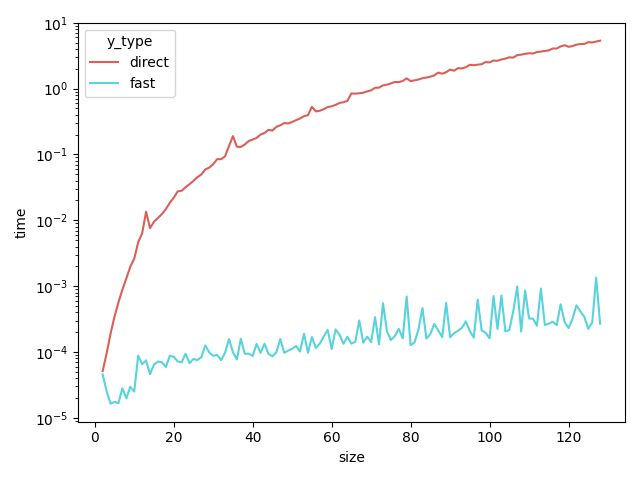
\includegraphics[width=0.8\textwidth]{../test/benchmark-results/bench-incremental-0.png}
	\caption{Confronto tra DCT diretta e veloce, sull'asse delle ascisse la
		dimensione delle metrici, sull'asse delle ordinate il tempo di esecuzione in
		scala logaritmica.}
	\label{fig:incremental-benchmark}
\end{figure}

Come si può osservare dal grafico in Figura
\ref{fig:incremental-benchmark}, il tempo computazione della DCT calcolata
tramite il metodo diretto cresce in maniera decisamente più rapida rispetto a
quello della DCT calcolata tramite la libreria \texttt{fft} di \texttt{scipy}.

La DCT2 calcolata tramite il metodo diretto presenta tempi proporzionali a $N^3$
rendendola quindi inutilizzabile per matrici di grandi dimensioni, la DCT calcolata
tramite la libreria \texttt{fft} di \texttt{scipy} invece presenta tempi di esecuzione 
decisamente migliori.

Siccome la libreria \texttt{fft} di \texttt{scipy} utilizza la FFT, si è scelto
di mettere a confronto i tempi di esecuzione della traformatata DCT2 su input di
dimensioni pari a potenze di 2 crescenti.

\begin{figure}[H]
	\centering
	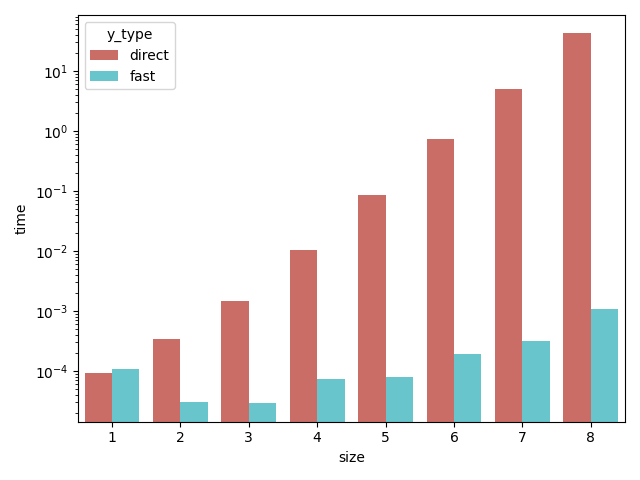
\includegraphics[width=0.8\textwidth]{../test/benchmark-results/bench-order-0.png}
	\caption{Confronto tra DCT diretta e veloce su input di dimensione pari a
		potenze di 2. Sull'asse delle ordinate il tempo in scala logaritmica,
		sull'asse delle ascisse le potenze di due delle dimensioni delle matrici.}
	\label{fig:order-benchmark}
\end{figure}

Anche in questo caso, come si può osservare dal grafico in figura
\ref{fig:order-benchmark}, la DCT implementata tramite il medoto diretto risulta
considerevolmente più lenta rispetto a quella implementata tramite la libreria
\texttt{fft} di \texttt{scipy}.

Tramite il software sviluppato è possibile ripetere i test qui presentati. Per
effettuare il confronto tra la DCT diretta che è stata implementata e quella
\textit{fast} di \texttt{scipy} su matrici di dimensione incrementali comprese
tra un valore di lower e upper buond, si può lanciare il programma con i
seguenti argomenti:
\vspace{12pt}
\begin{lstlisting}[frame=single]
 > python main.py --nogui \
			--performance --incremental --lower <value> --upper <value>
\end{lstlisting}

Il software sviluppato permette inoltre di eseguire il confronto sulle
prestazioni delle due trasformate su matrici di dimensioni pari a multipli di 2
tramite i seguenti comandi:
\vspace{12pt}
\begin{lstlisting}[frame=single]
 > python main.py --nogui \
      --performance --order --lower <value> --upper <value>
\end{lstlisting}

Siccome è stato necessario implementare la trasformata coseno diretta, al fine
di poterne verificare la corretta è stato necessario introdurre dei metodi di
test appositi. Si è scelto di esporre questi metodi tramite il parametro
\texttt{test}.

E' possibile quindi eseguire solo il test della corretta implementazione della
trasformata coseno con i seguenti parametri:
\vspace{12pt}
\begin{lstlisting}[frame=single]
 > python main.py --nogui --test
\end{lstlisting}

Per avere tutti i parametri con le loro descrizioni è possibile usare il
parametro \texttt{help} come segue:
\vspace{12pt}
\begin{lstlisting}[frame=single]
 > python main.py --help
    Cosine Image Compression,
    Written By Lorenzo Olearo and Alessandro Riva, 2023

    options:
      -h, --help            Show this help message and exit
      --nogui               Run program with no GUI
      --test                Run test
      --performance         Run performance test
      --slow                Use direct cosine transform [...]
      --order               Test DCT on matrix on order of 2 [...]
      --incremental         Test DCT on matrix on incremental [...]
      --lower LOWER         Lower bound for performance tests
      --upper UPPER         Upper bound for performance tests
      --iterations          Iteration of the same tests
      --load                Load pre-computed data in order to [...]
\end{lstlisting}




\section{Compressione di immagini}
La seconda parte della consegna richiede la realizzazione di un'interfaccia
grafica che permetta di caricare un'immagine in formato \texttt{BMP} in toni di
grigio e di applicare un algoritmo di compressione JPEG senza però utilizzare una
matrice di quantizzazione.

Anche per la realizzazione di questa seconda parte si è scelto di utilizzare
Python, in particolare, l'interfaccia grafica è stata realizzata tramite la
libreria \texttt{tkinter}.

Il software implementato permette all'utente di caricare un'immagine
\texttt{BMP} in scala di grigi dal proprio filesystem sfruttando il \textit{file
  picker} di \texttt{tkinter}.

Una volta caricata l'immagine all'interno dell'applicazione, l'utente è in grado
di specificare:

\begin{itemize}
  \item un intero $F$ corrispondente alla dimensione in pixel dei
        \textit{macro-blocchi} su cui effettuare la DCT2.
  \item un intero $d$ compreso tra $0$ e $2F - 2$ rappresentante il valore di
        taglio delle frequenza
\end{itemize}

Una volta trasfrormata l'immagine, l'applicazione mostra fianco a fianco
l'immagine originale e quella su cui è stato eseguito l'algoritmo di
compressione delle frequenze. L'applicazione permette inoltre \texttt{zoom} e
\texttt{pan} delle due immagini simultaneamente.

L'interfaccia grafica presenta una barra di controllo mostrata in 
figura~\ref{fig:control-bar} dove sono presenti due pulsanti, uno per 
selezionare l'immagine da utilizzare e uno per avviare il processo di 
compressione con DCT. Dopo il caricamento dell'immagine il pulsante per avviare 
la compressione viene abilitato insieme ai campi per l'input dei parametri 
$F$ e $d$.

\begin{figure}[h]
  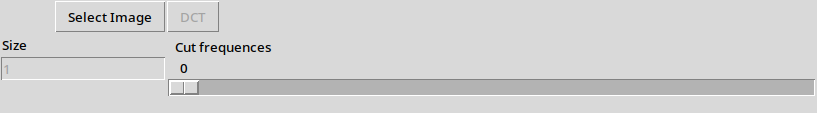
\includegraphics[width=\textwidth]{./imgs/control-bar.png}
  \caption{Barra di controllo dell'applicazione.}
  \label{fig:control-bar}
\end{figure}

L'inserimento del parametro $F$, è limitato ai valori tra 1 e la dimensione 
dell'immagine, e lo slider per il parametro $d$, è limitato tra $0$ e $2F-2$.
Alla pressione del pulsante DCT viene eseguita la trasformata e viene mostrato
il risultato della compressione affiancato all'immagine originale come mostrato
in figura~\ref{fig:after-transform}.

\begin{figure}[h]
  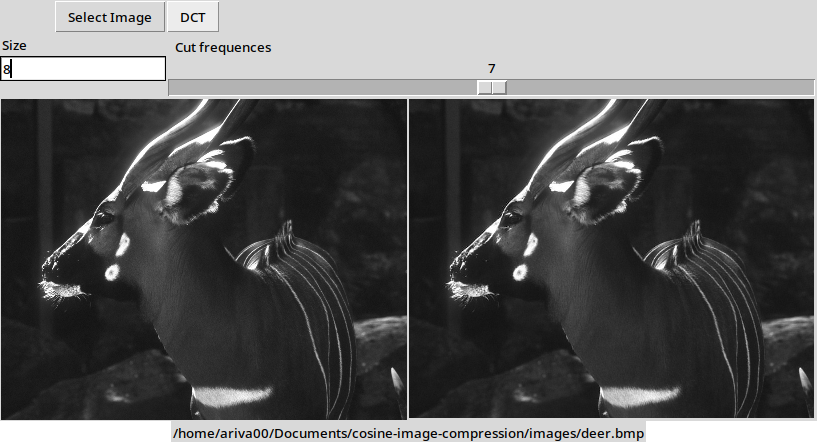
\includegraphics[width=\textwidth]{./imgs/after-transform.png}
  \caption{L'applicazione mostra l'immagine originale e quella trasformata.}
  \label{fig:after-transform}
\end{figure}

Per meglio visualizzare l'immagine è possibile utilizzare la rotella del mouse 
per scalarla e il tasto sinisto per trascinarla. Così facendo è possibile
apprezzare la differenza tra le due immagini come in 
figura~\ref{fig:zoomed-detail}.

\begin{figure}[h]
  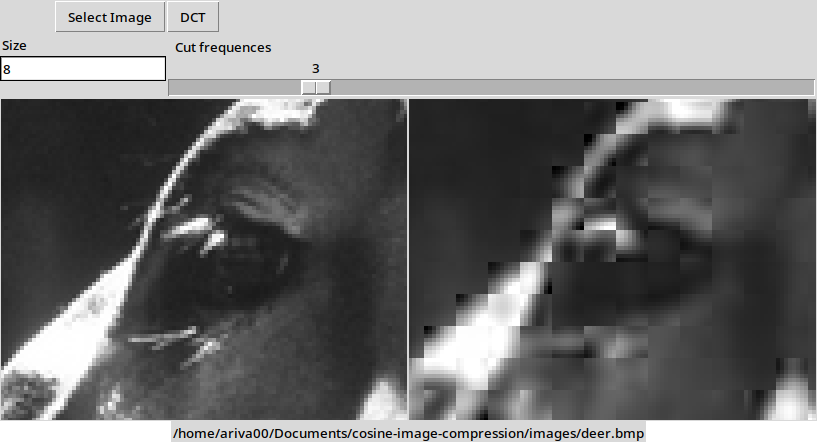
\includegraphics[width=\textwidth]{./imgs/zoomed-detail.png}
  \caption{Zoom su un dettaglio dell'immagine.}
  \label{fig:zoomed-detail}
\end{figure}

Lo zoom e il pan sono implementati tramite il modulo \texttt{PIL} di Python che
viene utilizzato per tagliare e ridimensionare le immagini prima di mostrarle, 
le trasformazioni utilizzano un criterio nearest neighbour, in modo da non 
introdurre artefatti durante lo zoom.

\end{document}
